\subsection{Motor Controller 1}
% Kabeláž
% add schematic and datasheet

\subsubsection{Description, type, operation parameters}
%Describe important functions; provide table with main parameters like resulting voltages->minimum, maximum, nominal, currents etc.
Motor controller is a prototype of MiRy X-Boss Motor Controller. It is fully self-designed for driving 2 PMSM motors simultaneously with Resolver sensors as a position feedback. Field Oriented Control is implemented with galvanic isolated current sensors LEM HTFS 200-P.

Galvanic isolation on PCB is shown in \ref{app:mc-top} and \ref{app:mc-bot}. The only place where isolation is smaller then required 4mm is between pins of DC/DC NME1215SC. Real space gap is 1.54mm. The NME1215SC has rated voltage of 1kV. See \ref{app:NME1215SC}.

Motor Controller communicate with traction control unit by private CAN bus. If any error occurs in their communication – Motor Controller stops driving both motors (error mode). It also implements discharge circuit which is activated by CAN or in case of Auxiliary supply disconnection (resistors are driven by normally-closed relay).

A current limit is set to not overload used motors. For each motor controller different. Rear motor controller has set peak current limit to 202A and temperature limit to 120°C. Front Motor Controller’s current limit is 70A and temperature limit also 120$\circ$C.

\begin{table}[H]
	\centering
	\caption{General motor controller data}
	\begin{tabularx}{\textwidth}{|X|X|}\hline
		Motor controller type: & MiRy X-Boss \\[\TableSize]\hline
		Maximum continous power: & 2 x 90kW (in:400V, out:200A) \\[\TableSize]\hline
		Maximum peak power: & 2 x 146kW for 5s (in:400V, out:300A) \\[\TableSize]\hline
		Maximum Input voltage: & 410VDC \\[\TableSize]\hline
		Output voltage: & 282 VAC \\[\TableSize]\hline
		Maximum continuous output current: & 2 x 200A \\[\TableSize]\hline
		Maximum peak current: & 2 x 300A for 5s \\[\TableSize]\hline
		Control method: & CAN \\[\TableSize]\hline
		Cooling method: & Water \\[\TableSize]\hline
		Auxiliary supply voltage: & 24VDC \\[\TableSize]\hline
	\end{tabularx}%
	\label{tab:MC:general}%
\end{table}%

\subsubsection{Wiring, cables, current calculations, connectors}
%Describe the wiring, show schematics, provide calculations for currents and voltages and show data regarding the cables and connectors used.

Motor controllers are connected with HVD box by high voltage cable. High current connector “ASHD 0 22-24320 P N” by Deutsch is used. 

\begin{table}[H]
	\centering
	\caption{Wire data of OLFLEX HEAT 180}
	\begin{tabularx}{\textwidth}{|X|X|}\hline
		Wire type: & OLFLEX HEAT 180 SiF  \\[\TableSize]\hline
		Current rating: & 165A \\[\TableSize]\hline
		Fuse current rating: & 160A \\[\TableSize]\hline
		Maximum operating voltage: & 500V \\[\TableSize]\hline
		Temperature rating: & 180 °C \\[\TableSize]\hline
	\end{tabularx}%
	\label{tab:MC:wire}%
\end{table}%

%table
\subsubsection{Position in car}
%Provide CAD-renderings showing the relevant parts. Mark the parts in the rendering, if necessary.

The position of both motor controllers is shown in \ref{fig:MC:position}.

\begin{figure}[H]
	\centering
	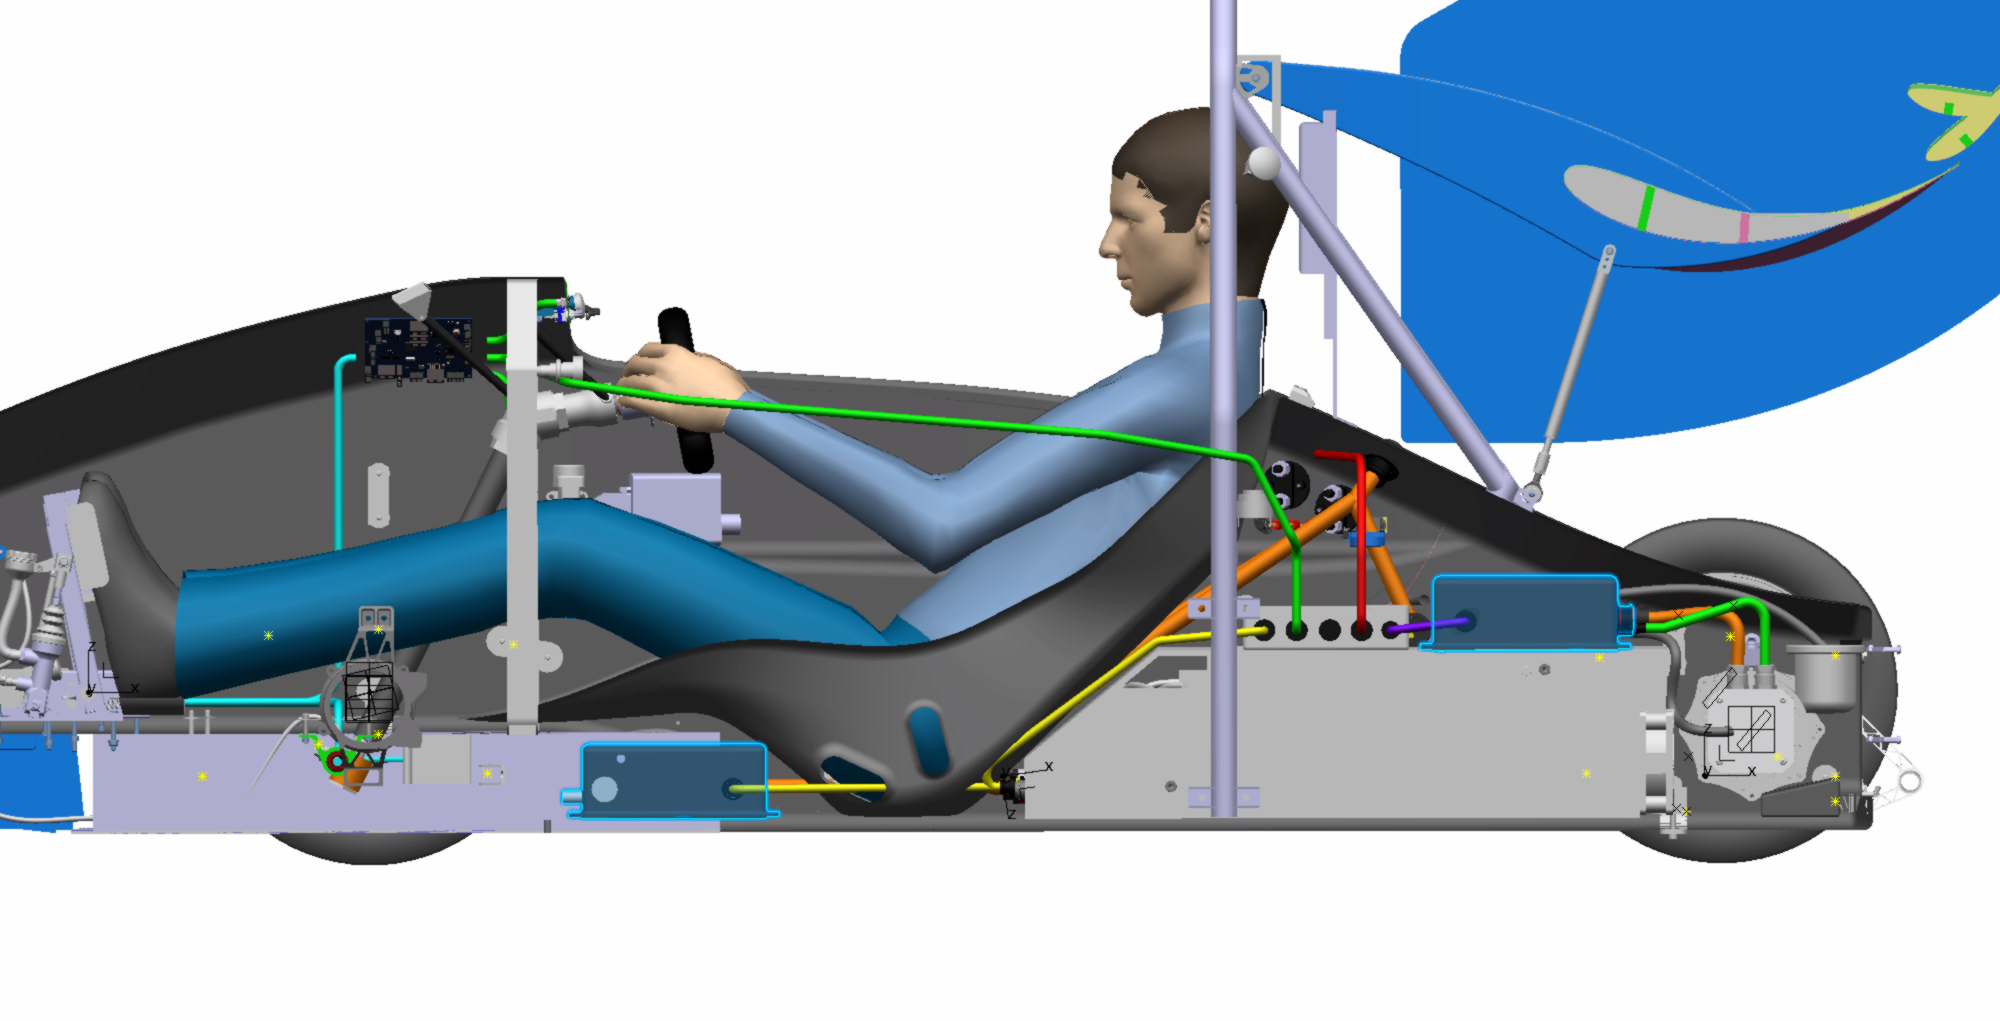
\includegraphics[width=\textwidth]{./img/MC-position.jpg}
	\caption{MC position.}
	\label{fig:MC:position}
\end{figure}
\subsection{Motor Controller 2}
%If identical parts are used, just refer to the corresponding sections, don’t copy and paste.
Motor controller 2 is identical as Motor controller 1.




